% =============================================================================
% SECCION: LA PARADOJA DEL DIRECTIONAL ACCURACY
% =============================================================================

\subsection{La Paradoja del \textit{Directional Accuracy}}
\label{sec:da_paradox}

En los datos analizados se observa una desconexi\'on entre el \textit{Directional Accuracy} (DA), la m\'etrica m\'as usada para evaluar predicciones de direcci\'on, y la rentabilidad, de modo que el DA no resulta un predictor confiable del rendimiento de una estrategia.

\subsubsection{Discrepancia entre Precisi\'on Direccional y Rentabilidad}
\label{subsec:counterintuitive}

Intuitivamente, un modelo que acierta m\'as la direcci\'on del mercado deber\'ia generar mayores retornos. Los resultados, sin embargo, no se alinean con esta expectativa.

\begin{equation}
\rho(\text{DA}, \text{Return}) = -0.37
\end{equation}

La correlaci\'on entre \textit{Directional Accuracy} y retorno total, computada sobre los 23 modelos y de car\'acter ilustrativo dado el tama\~no muestral reducido, es moderadamente negativa, lo que sugiere que modelos con mayor DA no generan necesariamente mejores retornos.

La Tabla~\ref{tab:da_paradox} presenta casos ilustrativos de esta paradoja.

\begin{table}[htbp]
\centering
\caption{Paradoja DA vs Retorno: Casos Ilustrativos}
\label{tab:da_paradox}
\begin{tabular}{@{}lrrr@{}}
\toprule
\textbf{Modelo} & \textbf{DA General} & \textbf{Retorno Total} & \textbf{Categor\'ia} \\
\midrule
GARCH & 54.3\% & +26.6\% & Alto DA, Retorno Modesto \\
Theta & 54.6\% & +44.4\% & Alto DA, Retorno Modesto \\
ExponentialSmoothing & 51.3\% & $-$15.4\% & Alto DA, Retorno Negativo \\
\midrule
LSTM+Attention & 47.0\% & +395\% & DA Bajo, Mejor Retorno \\
Ridge & 46.8\% & +253\% & DA Bajo, Alto Retorno \\
CNN-LSTM & 45.5\% & +122\% & DA Bajo, Alto Retorno \\
\bottomrule
\end{tabular}

\vspace{0.2cm}
\parbox{0.9\textwidth}{\footnotesize\textit{Nota: DA calculado como porcentaje de d\'ias donde la predicci\'on de direcci\'on coincide con el movimiento realizado del mercado.}}
\end{table}

\begin{figure}[htbp]
\centering
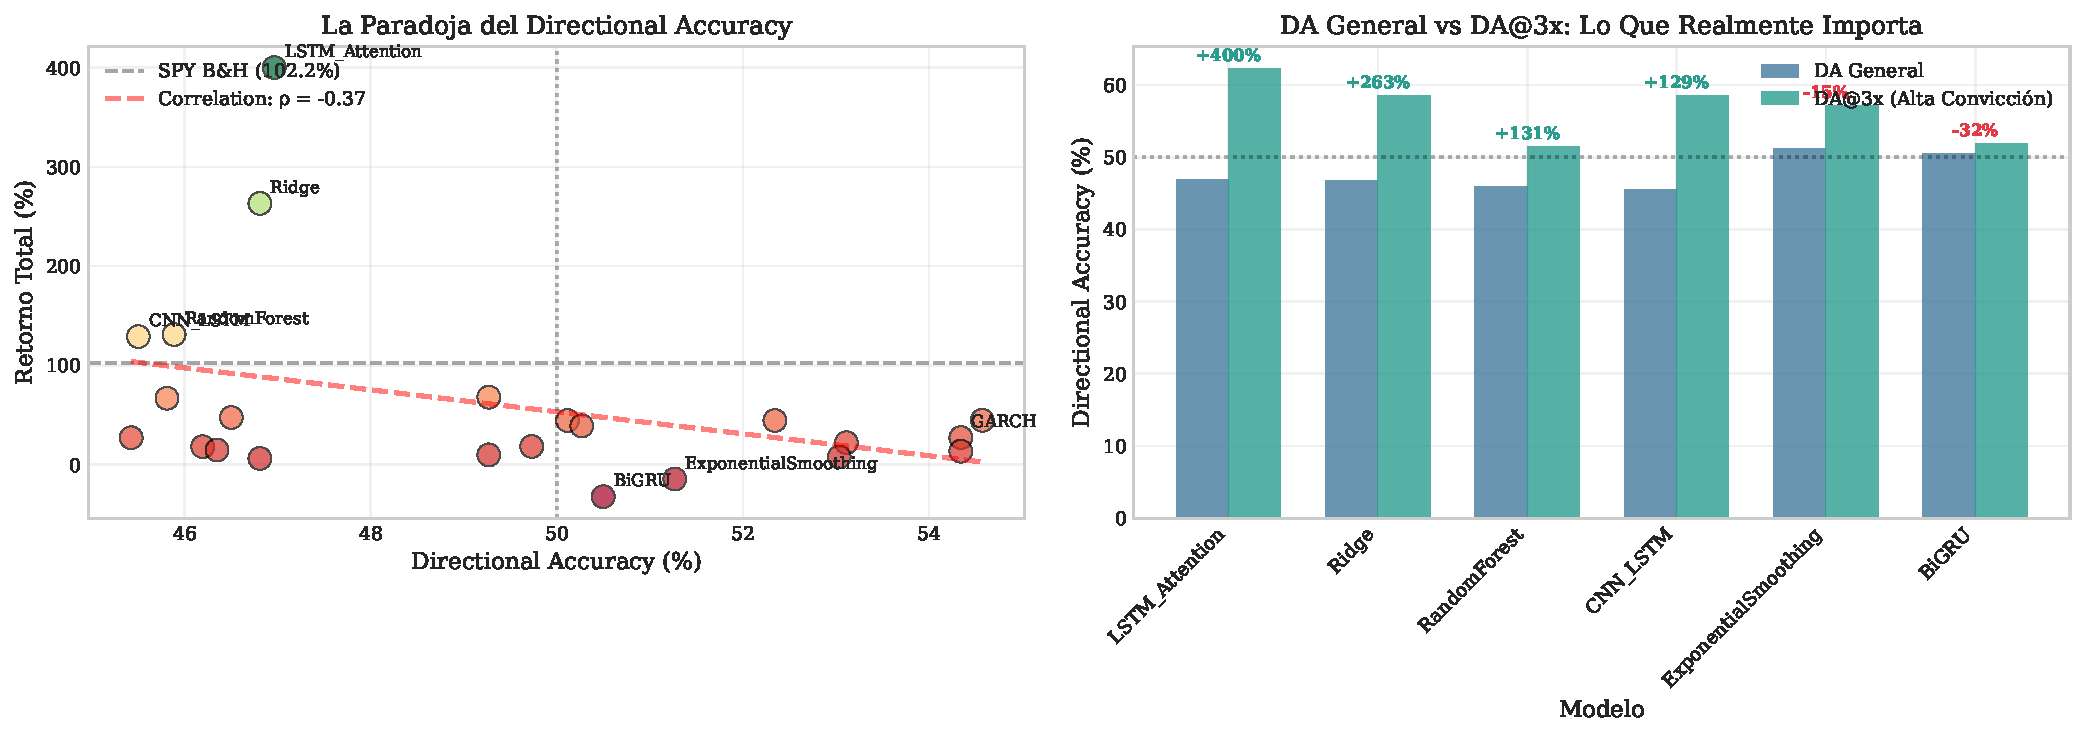
\includegraphics[width=\textwidth]{figures/da_vs_return_paradox.pdf}
\caption{La Paradoja del \textit{Directional Accuracy}. Panel izquierdo: \textit{Scatter plot} de DA vs Retorno Total mostrando correlaci\'on negativa ($\rho = -0.37$). Panel derecho: Comparaci\'on de DA General vs DA@3x (\textit{hit rate} en posiciones apalancadas) para modelos seleccionados. Los retornos se indican sobre cada par de barras.}
\label{fig:da_paradox}
\end{figure}

La Figura~\ref{fig:da_paradox} ilustra gr\'aficamente esta relaci\'on inversa entre precisi\'on direccional y rentabilidad.

\subsubsection{Factores de Rentabilidad no Capturados por el \textit{Directional Accuracy}}
\label{subsec:paradox_explanation}

El DA asigna el mismo peso a cada predicci\'on, sin distinguir entre la magnitud del movimiento, el tama\~no de la posici\'on o el momento del ciclo de mercado. El siguiente ejemplo ilustra esta limitaci\'on.

\begin{center}
\small
\begin{tabular}{@{}clcl@{}}
\toprule
\textbf{D\'ia} & \textbf{Movimiento} & \textbf{Predicci\'on} & \textbf{Resultado} \\
\midrule
1 & Mercado $+0.1\%$ & Correcta & \cmark \\
2 & Mercado $+0.1\%$ & Correcta & \cmark \\
3 & Mercado $-3.0\%$ & Incorrecta & \xmark \\
\bottomrule
\end{tabular}
\end{center}

\noindent DA = 66.7\% (2/3 aciertos), pero el P\&L acumulado es \textbf{negativo}, dado que la p\'erdida del d\'ia~3 ($-3.0\%$) supera las ganancias combinadas de los d\'ias~1 y~2 ($+0.2\%$).

La rentabilidad de una estrategia de \textit{trading} depende de tres factores que el DA no captura. En primer lugar, \textit{cu\'ando} se acierta, dado que acertar en d\'ias de movimientos grandes importa m\'as que acertar en d\'ias tranquilos, ya que el P\&L se determina por la magnitud del movimiento, no por haber acertado la direcci\'on. En segundo lugar, \textit{cu\'anto} se expone, ya que el tama\~no de la posici\'on cuando se acierta frente al tama\~no cuando se falla determina la contribuci\'on neta de cada predicci\'on al resultado. En tercer lugar, la asimetr\'ia entre ganancias y p\'erdidas, donde el ratio entre la ganancia promedio y la p\'erdida promedio por \textit{trade} (\hyperlink{glos:profit_factor}{\textit{Profit Factor}}) puede compensar una tasa de aciertos moderada si las ganancias son sustancialmente mayores que las p\'erdidas.

\subsubsection{Definici\'on del Indicador DA@3x}
\label{subsec:da_3x}

Se propone el indicador \textbf{DA@3x} (\textit{Directional Accuracy} en posiciones apalancadas) como una m\'etrica que podr\'ia resultar m\'as informativa sobre la rentabilidad en este contexto.

\begin{equation}
\text{DA@3x} = \frac{\displaystyle\sum_{t=1}^{T} \mathbf{1}\bigl[\text{pos}_t = 3 \;\wedge\; r_t^{\text{mkt}} > 0\bigr]}{\displaystyle\sum_{t=1}^{T} \mathbf{1}\bigl[\text{pos}_t = 3\bigr]}
\end{equation}

donde $\mathbf{1}[\cdot]$ es la funci\'on indicadora, $\text{pos}_t$ es la posici\'on asignada en el d\'ia $t$ y $r_t^{\text{mkt}}$ es el retorno del mercado en ese d\'ia. El numerador cuenta los d\'ias en los que el modelo mantiene la posici\'on apalancada m\'axima (UPRO, 3x) y el mercado efectivamente sube; el denominador cuenta el total de d\'ias en posici\'on 3x. As\'i, el DA@3x mide exclusivamente la precisi\'on del modelo en sus decisiones de mayor convicci\'on, es decir, aquellas en las que la exposici\'on y, por tanto, el impacto sobre el portafolio son m\'aximos. La Tabla~\ref{tab:da_vs_da3x} compara ambas m\'etricas para los modelos m\'as representativos.

\begin{table}[htbp]
\centering
\caption{Comparaci\'on entre DA General y DA@3x por modelo}
\label{tab:da_vs_da3x}
\begin{tabular}{@{}lrrrr@{}}
\toprule
\textbf{Modelo} & \textbf{DA General} & \textbf{DA@3x} & \textbf{\% Tiempo 3x} & \textbf{Retorno} \\
\midrule
LSTM+Attention & 47.0\% & 62.3\% & 12.2\% & +395\% \\
Ridge & 46.8\% & 58.5\% & 20.8\% & +253\% \\
RandomForest & 45.9\% & 51.5\% & 5.2\% & +128\% \\
CNN-LSTM & 45.5\% & 58.6\% & 12.1\% & +122\% \\
\midrule
GARCH & 54.3\% & 63.6\% & 1.7\% & +26.6\% \\
Theta & 54.6\% & 53.3\% & 2.3\% & +44.4\% \\
\bottomrule
\end{tabular}

\vspace{0.2cm}
\parbox{0.9\textwidth}{\footnotesize\textit{Nota: DA@3x = hit rate cuando el modelo est\'a en posici\'on 3x (UPRO). \% Tiempo 3x indica qu\'e fracci\'on del per\'iodo el modelo estuvo en posici\'on apalancada.}}
\end{table}

En esta muestra, los modelos con mejor rendimiento comparten tres caracter\'isticas interrelacionadas. En primer lugar, exhiben un DA@3x superior a su DA general; LSTM+Attention registra un 47.0\% de DA general pero un 62.3\% de DA@3x, lo que indica que, en el per\'iodo de prueba, su tasa de aciertos es mayor cuando asume mayor exposici\'on. En segundo lugar, son selectivos en el uso del apalancamiento; LSTM+Attention reserva la posici\'on 3x para el 12.2\% del tiempo, activ\'andola cuando las predicciones alcanzan los percentiles m\'as extremos. En tercer lugar, permanecen en efectivo cuando la se\~nal del modelo no alcanza los umbrales requeridos para tomar posici\'on, un 55\% del tiempo en el caso de LSTM+Attention. En contraste, GARCH presenta un DA@3x del 63.6\% (el m\'as alto del estudio), pero apenas asigna la posici\'on 3x el 1.7\% del tiempo, lo que limita su capacidad de generar retornos, a pesar de una precisi\'on condicional alta sobre un n\'umero reducido de observaciones. Theta (54.6\% DA general vs 53.3\% DA@3x) ejemplifica el caso opuesto, donde su precisi\'on direccional se concentra en movimientos de mercado de peque\~na magnitud que no compensan los errores en los d\'ias cr\'iticos.

\subsubsection{Implicaciones para el Dise\~no de Estrategias}
\label{subsec:strategy_implications}

Este hallazgo tiene implicaciones directas para el dise\~no de estrategias, dado que optimizar un modelo para maximizar el DA puede resultar contraproducente, ya que favorece modelos que aciertan frecuentemente en movimientos peque\~nos a costa de fallar en los d\'ias de mayor impacto. Resulta preferible evaluar los modelos mediante m\'etricas que capturen la asimetr\'ia condicional, como el \textit{Sharpe Ratio}, el \textit{Profit Factor} o el DA@3x propuesto en este estudio. El caso de LSTM+Attention resulta ilustrativo, ya que su DA general del 47.0\% lo descalificar\'ia bajo evaluaciones convencionales, pero su DA@3x del 62.3\% y su permanencia en efectivo el 55\% del tiempo coinciden con el retorno m\'as alto del estudio (+395\%), lo que sugiere que la rentabilidad observada se asocia m\'as con la concentraci\'on de aciertos en momentos de alta asimetr\'ia que con su frecuencia.


